% !TeX spellcheck = en_US
\chapter{Information Theory}
\label{cha:information-theory}
\todo{intro}

\section{Entropy}
\begin{align}
	&p(\textbf{x}) &&-\text{distribution (\eg over observation $\textbf{x}$)}\\
	\mathcal{H}(p) =& -\mathbb{E}_{\textbf{x}\sim p(\textbf{x})} [\log p(\textbf{x})] &&-\text{entropy - how "broad" $p(\textbf{x})$ is}\\
	=& - \sum_{i=1}^{N} p(\textbf{x}_i) \log p(\textbf{x}_i)
\end{align}

Intuition:
\begin{itemize}
	\item How \textit{random} is the variable?\\
	The more random the variable, the higher the entropy (\figref{fig:entropy})
	\item How large is the log \ac{prob} in expectation \textit{under} itself?
	\begin{itemize}
		\item If you mostly see low $\log$ \ac{prob}, then there are many places with similar \ac{prob}, and the entropy, as negative $\log$, would be high (\figref{fig:entropy-high}).
		\item If you mostly see high $\log$ \ac{prob}, then the variable focuses around only a few place, thus, the entropy, as negative $\log$, would be low (\figref{fig:entropy-low}).
	\end{itemize}	
\end{itemize}

\begin{figure}[hbt!]
	\centering
	\begin{subfigure}[b]{0.45\textwidth}
		\centering
		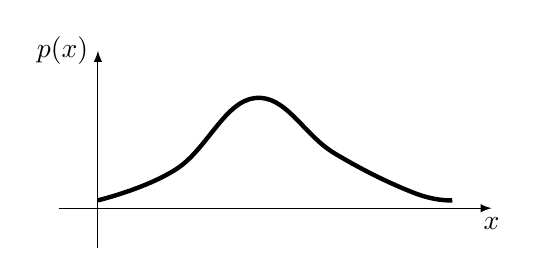
\begin{tikzpicture}
			\draw[-latex] (-.5,0) -- (5,0) node[below] {$x$};
			\draw[-latex] (0,-.5) -- (0,2) node[left] {$p(x)$};
			\draw[ultra thick] plot [smooth, tension=.7] coordinates {(0, 0.1) (1,0.5) (2,1.4) (3,0.7) (4, .2) (4.5,0.1)};
		\end{tikzpicture}
		\caption{Example of $p(x)$ with high entropy.}
		\label{fig:entropy-high}
	\end{subfigure}
	\hfill
	\begin{subfigure}[b]{0.45\textwidth}
		\centering
		\begin{tikzpicture}
			\draw[-latex] (-.5,0) -- (5,0) node[below] {$x$};
			\draw[-latex] (0,-.5) -- (0,2) node[left] {$p(x)$};
			\draw[ultra thick] plot [smooth, tension=.7] coordinates {(1.7,0.1) (2,1.4) (2.2,0.1)};
		\end{tikzpicture}
		\caption{Example of $p(x)$ with low entropy.}
		\label{fig:entropy-low}
	\end{subfigure}
	\caption{Examples of $p(x)$ with different entropy.}
	\label{fig:entropy}
\end{figure}

\section{Cross Entropy}
\label{sec:cross-entropy}
The cross entropy between two given \ac{prob} distributions $p$ and $q$ is defined as:
\begin{equation}
	H(p, q) = \mathbb{E}_p[-\log q]
\end{equation}
With \textbf{p, q} as discrete variables:
\begin{equation}
	H(\textbf{p, q}) = \sum_{i=1}^{C} p_i \log q_i
\end{equation}

\note $\nexists \log (0) \Rightarrow \text{condition: } \textbf{q} >0$

\section{Kullback - Leiber Divergence}

The \ac{KL}-divergence tells:
\begin{itemize}
	\item How \textit{different} are two distributions?
	\item How small is the expected log \ac{prob} of one distribution under another, \hlr{minus entropy}?
\end{itemize}

Example reference: 	\href{https://www.countbayesie.com/blog/2017/5/9/kullback-leibler-divergence-explained}{countbayesie}

\begin{align}
	H &= - \sum_{i=1}^{N} p(x_i) \log p(x_i)\\
	D_{KL}(p || q) &= \sum_{i=1}^N p(x_i) \left[ \log p(x_i) - \log q(x_i) \right]\\
	&= \sum_{i=1}^N p(x_i) \log \frac{p(x_i)}{q(x_i)}\\
	&= \mathbb{E}_{x \sim p(x)} \left[ \log p(x) - \log q(x) \right]
\end{align}
$\Rightarrow$ How many bits of info we expect to loose\\
$\Rightarrow$ \hlb{A function} that we can \hlb{optimized}

\textbf{\color{red} cross entropy = entropy + KL Divergence}
\begin{equation}
	{\color{red} H(p, q) = H(p) + D_{KL}(p || q)}
\end{equation}

\Eg: KL divergence between two normal distributions $\mathcal{N}(\mu_1, \sigma_1)$ and $\mathcal{N}(\mu_2, \sigma_2)$:
\begin{equation}
	D_{KL}(p, q) = \log \frac{\sigma_2}{\sigma_1} + \frac{\sigma_1^2 + (\mu_1 - \mu_2)^2}{2 \sigma_2^2} - \frac{1}{2}
\end{equation}

\underline{\textbf{PSEUDO CODE:}} with $\mu_2=0, \sigma_2 = 1$
\begin{align}
	\mu, \sigma &= \texttt{encoder}(\hat{x})\\
	\texttt{z} &= \mu + \sigma * \texttt{random\_normal(0, 1)}\\
	\texttt{y} &= \texttt{decoder(z)}\\
	\texttt{recon\_loss} &= \texttt{x.log(y) + (1-x)log(1-y)}\\
	\texttt{KL\_loss} &= \frac{1}{2} [ \mu^2 + \sigma^2 - \texttt{log}(\sigma^2 + 1e^{-8}) -1 ]\\
	\texttt{ELBO} &= \texttt{recon\_loss - KL\_loss}\\
	\texttt{loss} &= \texttt{-ELBO}
\end{align}

\section{Mutual Information}
\begin{align}
	&p(x) &&-\text{distribution (\eg over observation $\textbf{x}$)}\\
	\mathcal{H}(p(\textbf{x})) =& -\mathbb{E}_{\textbf{x}\sim p(\textbf{x})} [\log p(\textbf{x})] &&-\text{entropy - how "broad" $p(\textbf{x})$ is}\\
	\mathcal{I}(\textbf{x};\textbf{y}) =& D_{KL} \big(p(\textbf{x,y}) || p(\textbf{x}) p(\textbf{y})\big) &&-\text{mutual information}\\
	=& \mathbb{E}_{(\textbf{x,y}) \sim p(\textbf{x,y})} \left[ \log \frac{p(\textbf{x,y})}{p(\textbf{x})p(\textbf{y})} \right]\\
	=& \mathcal{H}(p(\textbf{y})) - \mathcal{H}(p(\textbf{y|x})) &&-\text{relates to \ac{IG}}
\end{align}
The last equation implies that we can interpret mutual information $\mathcal{I}(\textbf{x};\textbf{y})$ as \ac{IG}, how much more do we know about \textbf{y} after receiving observation about \textbf{x}.

\Eg:
\begin{itemize}
	\item If \textbf{x} and \textbf{y} are independent of each others, then $p(\textbf{x,y}) = p(\textbf{x}) p(\textbf{y})$, thus $\mathcal{I}(\textbf{x};\textbf{y})=0$
	\item If \textbf{x} and \textbf{y} depends on each others more and more, the different between the joint \ac{prob} $p(\textbf{x,y})$ and the product of marginal \ac{prob} $p(\textbf{x}) p(\textbf{y})$ grows, thus the $\mathcal{I}(\textbf{x};\textbf{y})$ is larger.
\end{itemize}